% Merged visual account approved in CX-74--CX-79.  The numerical example is
% generated by joint_tutorial_worked_example.py.  Receiver actions follow
% Algorithms 1--5 of juna_joint_ieee.tex.
\documentclass[aspectratio=169,10pt]{beamer}
\usepackage[T1]{fontenc}
\usepackage{amsmath,amssymb,amsfonts}
\usepackage{bm}
\usepackage{tikz}
\usepackage{xcolor}
\usetikzlibrary{arrows.meta,positioning,shapes,calc}

\definecolor{parchment}{HTML}{F4E8C8}
\definecolor{paper}{HTML}{FAF1D8}
\definecolor{ink}{HTML}{1A1A1A}
\definecolor{inkgray}{HTML}{5A5A5A}
\definecolor{accentred}{HTML}{8B1A1A}
\definecolor{accentgreen}{HTML}{2D5F2C}
\definecolor{accentblue}{HTML}{1F4E79}
\definecolor{redbg}{HTML}{F7E0DE}
\definecolor{grnbg}{HTML}{E0EBDC}
\definecolor{blubg}{HTML}{DDE6EF}
\definecolor{labelbg}{HTML}{EFE0B0}

\usefonttheme{serif}
\setbeamercolor{background canvas}{bg=parchment}
\setbeamercolor{normal text}{fg=ink}
\setbeamercolor{structure}{fg=ink}
\setbeamercolor{frametitle}{fg=ink,bg=parchment}
\setbeamercolor{title}{fg=ink}
\setbeamercolor{itemize item}{fg=ink}
\setbeamercolor{itemize subitem}{fg=ink}
\setbeamercolor{item}{fg=ink}
\setbeamercolor{caption name}{fg=ink}
\setbeamertemplate{navigation symbols}{}
\setbeamertemplate{itemize item}{\textbullet}

\setbeamertemplate{frametitle}{%
  \vspace{0.30em}%
  \begin{center}%
    {\bfseries\Large\insertframetitle\par}%
    \vspace{0.28em}%
    {\color{ink}\rule{0.86\paperwidth}{0.4pt}}%
  \end{center}%
  \vspace{0.10em}%
}
\setbeamertemplate{footline}{%
  \hbox to \paperwidth{\hfil\itshape\small\insertframenumber\hspace{0.7em}}%
  \vspace{0.35em}%
}

\newcommand{\vY}{\bm{Y}}
\newcommand{\vy}{\bm{y}}
\newcommand{\vA}{\bm{A}}
\newcommand{\vB}{\bm{B}}
\newcommand{\valpha}{\bm{\alpha}}
\newcommand{\vn}{\bm{n}}
\newcommand{\vs}{\bm{s}}
\newcommand{\vW}{\bm{W}}
\newcommand{\T}{^{\mathsf T}}
\newcommand{\Hh}{^{\mathsf H}}
\newcommand{\norm}[1]{\left\lVert #1\right\rVert}
\DeclareMathOperator*{\argmin}{arg\,min}

\tikzset{
  flowbox/.style={draw=ink,fill=paper,line width=0.6pt,
                  minimum width=2.5cm,minimum height=1.0cm,
                  align=center,font=\small\bfseries,inner sep=4pt},
  smallbox/.style={draw=ink,fill=paper,line width=0.4pt,
                   minimum width=0.7cm,minimum height=0.55cm,
                   inner sep=2pt,align=center,font=\footnotesize\itshape},
  method/.style={draw=accentgreen,fill=grnbg,line width=1.0pt,
                 align=center,font=\small\bfseries,inner sep=6pt},
  issue/.style={draw=accentred,fill=redbg,line width=1.0pt,
                align=center,font=\small\bfseries,inner sep=6pt},
  idea/.style={draw=accentblue,fill=blubg,line width=1.0pt,
               align=center,font=\small\bfseries,inner sep=6pt},
  flowarr/.style={-{Stealth[length=2.5mm,width=2mm]},line width=0.7pt},
  softarr/.style={-{Stealth[length=2mm,width=1.6mm]},line width=0.5pt,color=inkgray}
}

\newcommand{\bottomnote}[1]{%
  \begin{center}{\itshape\small #1}\end{center}}

\newcommand{\papercover}[4]{%
  \begin{frame}[plain]
    \vfill
    \begin{center}
      {\bfseries\Huge #1\par}
      \vspace{0.8cm}
      {\Large #2\par}
      \vspace{0.35cm}
      {\itshape\large\color{inkgray}#3\par}
      \vspace{0.55cm}
      {\small\texttt{\detokenize{#4}}\par}
    \end{center}
    \vfill
  \end{frame}}

\newcommand{\twocolmodel}[4]{%
  \begin{columns}[T,onlytextwidth]
    \begin{column}{0.48\textwidth}#1\end{column}
    \begin{column}{0.48\textwidth}#2\end{column}
  \end{columns}
  \bottomnote{#3\\#4}}


\usetikzlibrary{fit,decorations.pathreplacing}

\newcommand{\Kset}{\mathcal K}
\newcommand{\Bset}{\mathcal B}
\newcommand{\Pset}{\mathcal P}
\newcommand{\E}{\mathbb E}
\newcommand{\Cfield}{\mathbb C}

\tikzset{
  card/.style={draw=ink,fill=paper,line width=0.55pt,rounded corners=2pt,
               align=center,inner sep=5pt,font=\small},
  goodcard/.style={draw=accentgreen,fill=grnbg,line width=0.85pt,
                   rounded corners=2pt,align=center,inner sep=5pt,font=\small},
  badcard/.style={draw=accentred,fill=redbg,line width=0.85pt,
                  rounded corners=2pt,align=center,inner sep=5pt,font=\small},
  bluecard/.style={draw=accentblue,fill=blubg,line width=0.85pt,
                   rounded corners=2pt,align=center,inner sep=5pt,font=\small},
  ghostcard/.style={draw=inkgray!65,fill=paper,line width=0.55pt,dashed,
                    rounded corners=2pt,align=center,inner sep=5pt,
                    font=\small,text=inkgray},
  panel/.style={draw=ink,fill=parchment,line width=0.9pt,rounded corners=3pt},
  matrixcell/.style={draw=inkgray!65,line width=0.25pt,
                     minimum width=0.36cm,minimum height=0.36cm,
                     inner sep=0pt},
  vcell/.style={draw=ink,fill=paper,line width=0.55pt,
                minimum width=1.05cm,minimum height=0.58cm,
                inner sep=1pt,font=\small},
  redarr/.style={-{Stealth[length=2.5mm,width=2mm]},line width=0.85pt,
                  draw=accentred},
  greenarr/.style={-{Stealth[length=2.5mm,width=2mm]},line width=0.85pt,
                    draw=accentgreen},
  bluearr/.style={-{Stealth[length=2.5mm,width=2mm]},line width=0.85pt,
                   draw=accentblue},
  grayarr/.style={-{Stealth[length=2.2mm,width=1.8mm]},line width=0.65pt,
                   draw=inkgray},
  cpbrace/.style={decorate,decoration={brace,amplitude=5pt,raise=2pt},
                  line width=0.6pt,color=inkgray}
}

\begin{document}

% =====================================================================
% 1. Cover
% =====================================================================
\begin{frame}[plain]
  \centering
  \vspace{0.18cm}
  {\small\color{inkgray}\texttt{juna\_joint\_ieee.tex}, in pictures\par}
  \vspace{0.14cm}
  {\bfseries\Huge The Joint Demodulation and Decoding Problem\par}
  \vspace{0.12cm}
  {\Large Carrier 4 inside the frame-wide receiver\par}
  \vspace{0.38cm}

  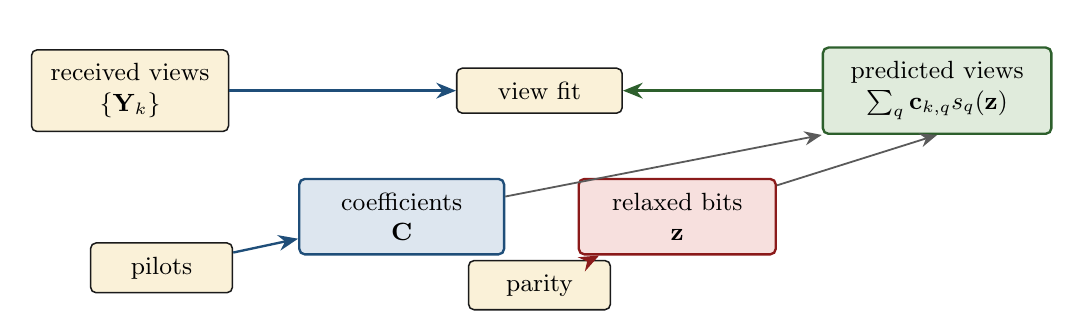
\begin{tikzpicture}[x=1cm,y=1cm]
    \path[use as bounding box] (-6.5,-1.85) rectangle (6.5,1.55);
    \node[card,text width=2.15cm] (views) at (-5.20,0.75)
      {received views\\$\{\mathbf Y_k\}$};
    \node[card,text width=1.75cm] (fit) at (0,0.75)
      {view fit};
    \node[goodcard,text width=2.55cm] (pred) at (5.05,0.75)
      {predicted views\\$\sum_q\mathbf c_{k,q}s_q(\mathbf z)$};
    \node[bluecard,text width=2.25cm] (coef) at (-1.75,-0.85)
      {coefficients\\$\mathbf C$};
    \node[badcard,text width=2.15cm] (bits) at (1.75,-0.85)
      {relaxed bits\\$\mathbf z$};
    \draw[bluearr] (views) -- (fit);
    \draw[greenarr] (pred) -- (fit);
    \draw[grayarr] (coef) -- (pred.south west);
    \draw[grayarr] (bits) -- (pred.south);

    \node[card,text width=1.45cm] (pilots) at (-4.80,-1.50) {pilots};
    \node[card,text width=1.45cm] (parity) at (0,-1.72) {parity};
    \draw[bluearr] (pilots) -- (coef);
    \draw[redarr] (parity) -- (bits);
  \end{tikzpicture}

  \vspace{0.10cm}
  {\small\color{inkgray}The combiner is a read-out.  The joint problem
   scores the coefficients and relaxed bits against the received views.\par}
\end{frame}

% =====================================================================

% 2. One-tap model
% =====================================================================
\begin{frame}{One-tap model}
  \begin{columns}[T,onlytextwidth]
    \begin{column}{0.47\textwidth}
      \centering
      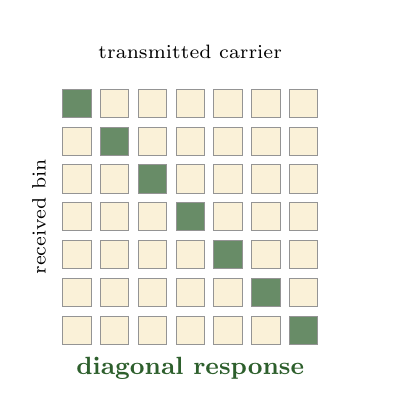
\begin{tikzpicture}[x=0.48cm,y=0.48cm]
        \path[use as bounding box] (-1.3,-1.4) rectangle (7.8,8.0);
        \foreach \r in {0,...,6}{
          \foreach \c in {0,...,6}{
            \node[matrixcell,fill=paper] at (\c,6-\r) {};
          }
          \node[matrixcell,fill=accentgreen!72] at (\r,6-\r) {};
        }
        \node[font=\scriptsize] at (3,7.35) {transmitted carrier};
        \node[font=\scriptsize,rotate=90] at (-1.0,3) {received bin};
        \node[font=\small\bfseries\color{accentgreen}] at (3,-1.0)
          {diagonal response};
      \end{tikzpicture}
    \end{column}
    \begin{column}{0.51\textwidth}
      \vspace{0.45cm}
      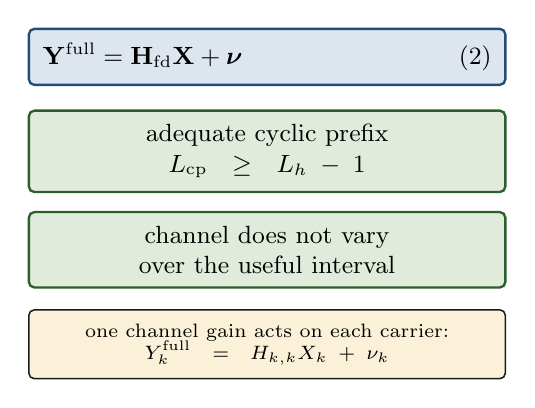
\begin{tikzpicture}
        \node[bluecard,text width=5.7cm] at (0,1.35)
          {$\mathbf Y^{\mathrm{full}}=\mathbf H_{\mathrm{fd}}\mathbf X+\bm\nu$
           \hfill\textnormal{(2)}};
        \node[goodcard,text width=5.7cm] at (0,0.15)
          {adequate cyclic prefix\\$L_{\rm cp}\ge L_h-1$};
        \node[goodcard,text width=5.7cm] at (0,-1.10)
          {channel does not vary\\over the useful interval};
        \node[card,text width=5.7cm,font=\scriptsize] at (0,-2.30)
          {one channel gain acts on each carrier:\\
           $Y_k^{\mathrm{full}}=H_{k,k}X_k+\nu_k$};
      \end{tikzpicture}
    \end{column}
  \end{columns}
  \bottomnote{Under both conditions, the fast Fourier transform diagonalizes the block channel and one pilot-specified equalizer tap per carrier suffices.}
\end{frame}

% =====================================================================
% 3. Same-symbol ICI
% =====================================================================
\begin{frame}{Same-symbol ICI}
  \centering
  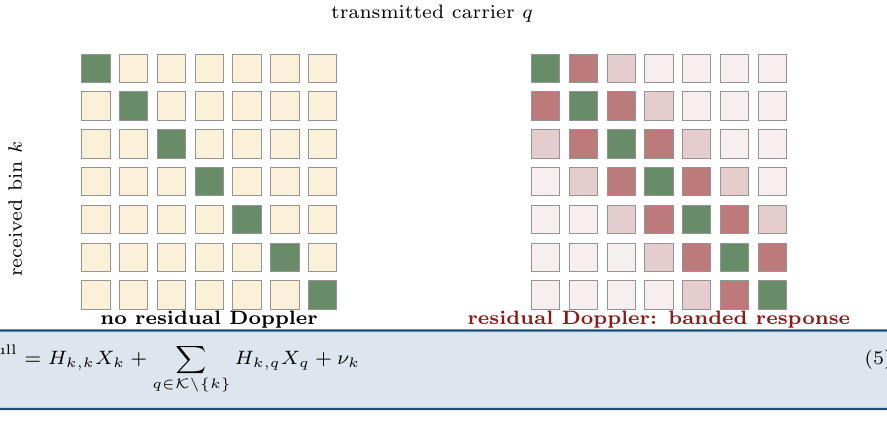
\begin{tikzpicture}[x=0.48cm,y=0.48cm]
    \path[use as bounding box] (-7.0,-2.1) rectangle (15.0,7.8);
    \begin{scope}[shift={(-5.2,0)},yshift=0.35cm]
      \foreach \r in {0,...,6}{
        \foreach \c in {0,...,6}{
          \node[matrixcell,fill=paper] at (\c,6-\r) {};
        }
        \node[matrixcell,fill=accentgreen!72] at (\r,6-\r) {};
      }
      \node[font=\scriptsize\bfseries,align=center] at (3,-0.65)
        {no residual Doppler};
    \end{scope}

    \uncover<2->{%
      \begin{scope}[shift={(6.7,0)},yshift=0.35cm]
        \foreach \r in {0,...,6}{
          \foreach \c in {0,...,6}{
            \pgfmathtruncatemacro{\dist}{abs(\r-\c)}
            \ifnum\dist=0
              \node[matrixcell,fill=accentgreen!72] at (\c,6-\r) {};
            \else\ifnum\dist=1
              \node[matrixcell,fill=accentred!58] at (\c,6-\r) {};
            \else\ifnum\dist=2
              \node[matrixcell,fill=accentred!22] at (\c,6-\r) {};
            \else
              \node[matrixcell,fill=accentred!7] at (\c,6-\r) {};
            \fi\fi\fi
          }
        }
        \node[font=\scriptsize\bfseries\color{accentred},align=center] at (3,-0.65)
          {residual Doppler: banded response};
      \end{scope}
    }
    \node[font=\scriptsize,yshift=0.35cm] at (3.7,7.45) {transmitted carrier $q$};
    \node[font=\scriptsize,rotate=90,yshift=0.35cm] at (-6.6,3) {received bin $k$};
    \uncover<2->{%
      \node[bluecard,text width=11.7cm,font=\scriptsize] at (3.7,-1.25) {
        $\displaystyle Y_k^{\mathrm{full}}
         =H_{k,k}X_k+\sum_{q\in\Kset\setminus\{k\}}H_{k,q}X_q+\nu_k$
        \hfill\textnormal{(5)}};
    }
  \end{tikzpicture}
  \bottomnote{\scriptsize The same symbol index with a different carrier index gives intercarrier interference (ICI).  Residual Doppler makes the frequency-domain operator non-diagonal.  For small residual Doppler and carrier-frequency offset, the coefficients remain near the diagonal and motivate a banded operator.}
\end{frame}

% =====================================================================
% 4. Short cyclic prefix
% =====================================================================
\begin{frame}{Insufficient cyclic prefix}
  \centering
  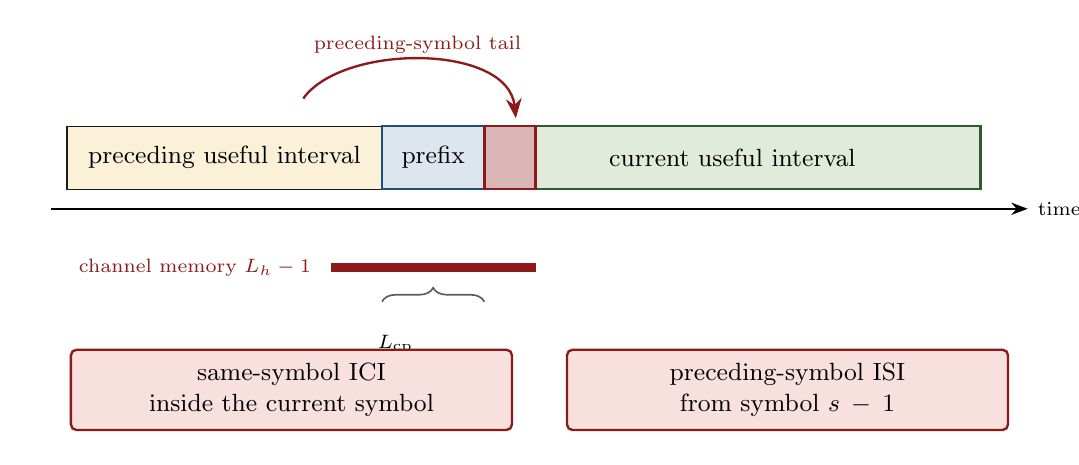
\begin{tikzpicture}[x=1cm,y=1cm,>=Stealth]
    \path[use as bounding box] (-6.5,-2.65) rectangle (6.5,2.55);
    \draw[->,line width=0.65pt] (-6.2,0.25) -- (6.2,0.25)
      node[right,font=\scriptsize] {time};
    \draw[fill=paper,draw=ink] (-6.0,0.50) rectangle (-2.0,1.30);
    \node[font=\small] at (-4.0,0.90) {preceding useful interval};
    \draw[fill=blubg,draw=accentblue,line width=0.9pt]
      (-2.0,0.50) rectangle (-0.7,1.30);
    \node[font=\small] at (-1.35,0.90) {prefix};
    \draw[fill=grnbg,draw=accentgreen,line width=0.9pt]
      (-0.7,0.50) rectangle (5.6,1.30);
    \node[font=\small] at (2.45,0.90) {current useful interval};

    \draw[accentred,line width=3.2pt] (-2.65,-0.50) -- (-0.05,-0.50);
    \node[font=\scriptsize\color{accentred},anchor=east] at (-2.78,-0.50)
      {channel memory $L_h-1$};
    \draw[cpbrace] (-2.0,-1.00) -- (-0.7,-1.00);
    \node[font=\scriptsize,anchor=east] at (-1.48,-1.47) {$L_{\rm cp}$};
    \fill[accentred!32] (-0.7,0.50) rectangle (-0.05,1.30);
    \draw[accentred,line width=1.0pt] (-0.7,0.50) rectangle (-0.05,1.30);
    \draw[redarr] (-3.0,1.65)
      .. controls (-2.5,2.35) and (-0.4,2.35) .. (-0.30,1.40);
    \node[font=\scriptsize\color{accentred}] at (-1.55,2.33)
      {preceding-symbol tail};

    \node[badcard,text width=5.25cm] at (-3.15,-2.05)
      {same-symbol ICI\\inside the current symbol};
    \node[badcard,text width=5.25cm] at (3.15,-2.05)
      {preceding-symbol ISI\\from symbol $s-1$};
  \end{tikzpicture}
  \vspace{-0.12cm}
  \bottomnote{\scriptsize A tap beyond the prefix carries the preceding symbol into the useful interval.  Different carriers in one symbol give ICI; different symbol indices give ISI.}
\end{frame}

% =====================================================================
% 5. Scope boundary
% =====================================================================
\begin{frame}{Model scope}
  \centering
  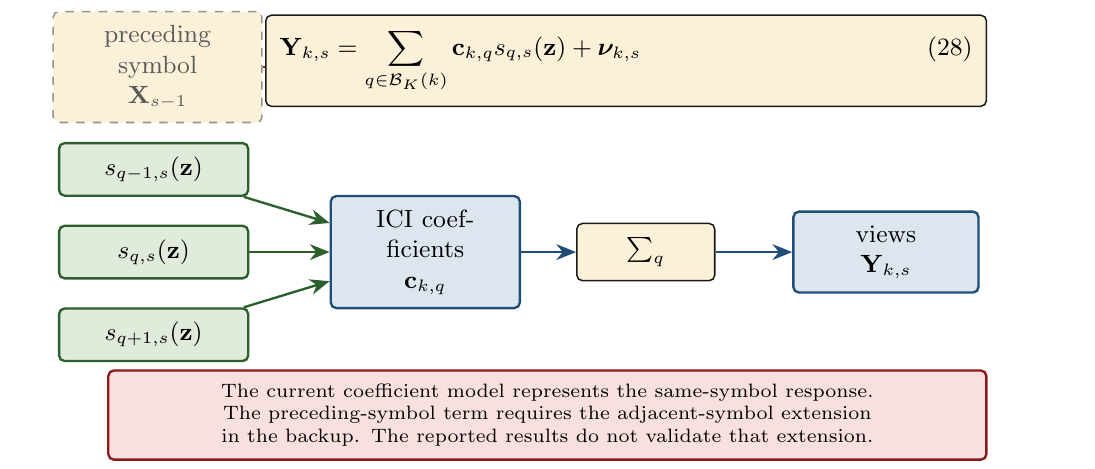
\begin{tikzpicture}[x=1cm,y=1cm]
    \path[use as bounding box] (-6.6,-2.80) rectangle (6.6,2.45);
    \node[goodcard,text width=2.05cm] (q1) at (-5.0,0.65)
      {$s_{q-1,s}(\mathbf z)$};
    \node[goodcard,text width=2.05cm] (q2) at (-5.0,-0.40)
      {$s_{q,s}(\mathbf z)$};
    \node[goodcard,text width=2.05cm] (q3) at (-5.0,-1.45)
      {$s_{q+1,s}(\mathbf z)$};
    \node[bluecard,text width=2.05cm] (resp) at (-1.55,-0.40)
      {ICI coefficients\\$\mathbf c_{k,q}$};
    \node[card,text width=1.40cm] (sum) at (1.25,-0.40) {$\sum_q$};
    \node[bluecard,text width=2.00cm] (obs) at (4.30,-0.40)
      {views\\$\mathbf Y_{k,s}$};
    \draw[greenarr] (q1) -- (resp);
    \draw[greenarr] (q2) -- (resp);
    \draw[greenarr] (q3) -- (resp);
    \draw[bluearr] (resp) -- (sum);
    \draw[bluearr] (sum) -- (obs);

    \node[ghostcard,text width=2.30cm] (previous) at (-4.95,1.95)
      {preceding symbol\\$\mathbf X_{s-1}$};
    \draw[redarr,dashed] (previous.east) -- ++(1.4,0)
      node[right,font=\scriptsize\color{accentred},align=left]
      {preceding-symbol term\\not represented};

    \node[card,text width=8.80cm] at (1.00,2.03) {
      $\displaystyle
       \mathbf Y_{k,s}=\sum_{q\in\Bset_K(k)}
       \mathbf c_{k,q}s_{q,s}(\mathbf z)+\bm\nu_{k,s}$
      \hfill\textnormal{(28)}};
    \node[badcard,text width=10.80cm,font=\scriptsize] at (0,-2.47)
      {The current coefficient model represents the same-symbol response.
       The preceding-symbol term requires the adjacent-symbol extension in the backup.
       The reported results do not validate that extension.};
  \end{tikzpicture}
\end{frame}

% =====================================================================
% 6. Running example
% =====================================================================
\begin{frame}{Worked example}
  \centering
  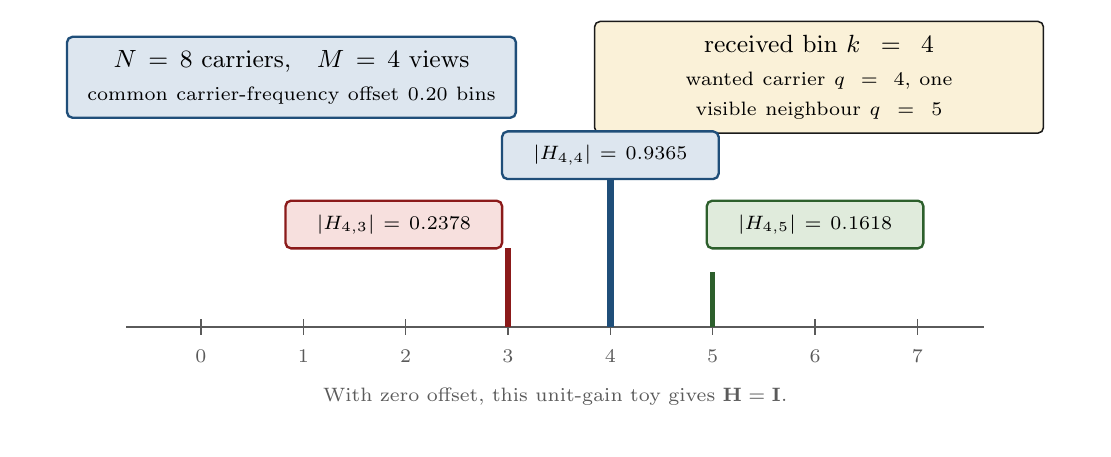
\begin{tikzpicture}[x=1cm,y=1cm]
    \path[use as bounding box] (-6.7,-2.75) rectangle (6.7,2.35);
    \node[bluecard,text width=5.35cm] at (-3.35,1.72)
      {$N=8$ carriers,\quad $M=4$ views\\[0.08em]
       \scriptsize common carrier-frequency offset $0.20$ bins};
    \node[card,text width=5.35cm] at (3.35,1.72)
      {received bin $k=4$\\[0.08em]
       \scriptsize wanted carrier $q=4$, one visible neighbour $q=5$};

    \draw[line width=0.6pt,color=inkgray] (-5.45,-1.45) -- (5.45,-1.45);
    \foreach \x/\lab in {-4.5/0,-3.2/1,-1.9/2,-0.6/3,0.7/4,2.0/5,3.3/6,4.6/7}{
      \draw[line width=0.5pt,color=inkgray] (\x,-1.55) -- (\x,-1.35);
      \node[font=\scriptsize,color=inkgray] at (\x,-1.82) {\lab};
    }
    \draw[line width=2.0pt,color=accentred] (-0.6,-1.45) -- (-0.6,-0.45);
    \draw[line width=2.5pt,color=accentblue] (0.7,-1.45) -- (0.7,0.55);
    \draw[line width=2.0pt,color=accentgreen] (2.0,-1.45) -- (2.0,-0.75);
    \node[badcard,text width=2.40cm,font=\scriptsize] at (-2.05,-0.15)
      {$|H_{4,3}|=0.2378$};
    \node[bluecard,text width=2.40cm,font=\scriptsize] at (0.70,0.73)
      {$|H_{4,4}|=0.9365$};
    \node[goodcard,text width=2.40cm,font=\scriptsize] at (3.30,-0.15)
      {$|H_{4,5}|=0.1618$};
    \node[font=\scriptsize,color=inkgray] at (0,-2.33)
      {With zero offset, this unit-gain toy gives $\mathbf H=\mathbf I$.};
  \end{tikzpicture}
  \vspace{-0.10cm}
  \bottomnote{\scriptsize The running example keeps carrier $4$, its four views, and carrier $5$ visible; the complete calculation retains all eight carriers.  It uses one OFDM symbol for an ICI example, not a measured Red channel or an ISI example.}
\end{frame}

% =====================================================================
% 7. Partial-FFT views
% =====================================================================
\begin{frame}{Partial-FFT views}
  \centering
  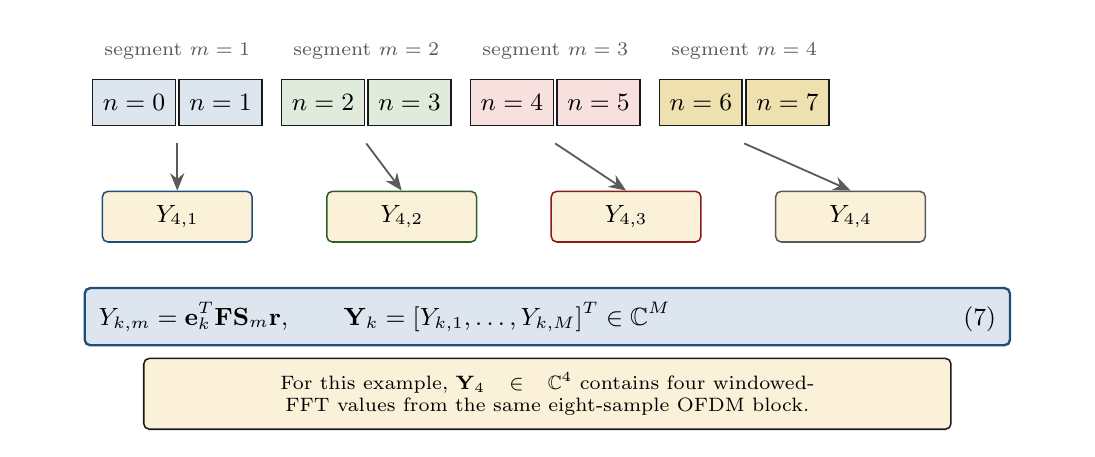
\begin{tikzpicture}[x=1cm,y=1cm]
    \path[use as bounding box] (-6.6,-2.75) rectangle (6.6,2.35);
    \foreach \x/\n/\fillcol in {
      -5.25/0/blubg,-4.15/1/blubg,
      -2.85/2/grnbg,-1.75/3/grnbg,
      -0.45/4/redbg,0.65/5/redbg,
      1.95/6/labelbg,3.05/7/labelbg}{
      \node[vcell,fill=\fillcol] at (\x,1.40) {$n=\n$};
    }
    \node[font=\scriptsize,color=inkgray] at (-4.70,2.05) {segment $m=1$};
    \node[font=\scriptsize,color=inkgray] at (-2.30,2.05) {segment $m=2$};
    \node[font=\scriptsize,color=inkgray] at (0.10,2.05) {segment $m=3$};
    \node[font=\scriptsize,color=inkgray] at (2.50,2.05) {segment $m=4$};

    \uncover<2->{%
      \foreach \m/\x/\col in {1/-4.70/accentblue,2/-1.85/accentgreen,3/1.00/accentred,4/3.85/inkgray}{
        \node[card,draw=\col,text width=1.55cm] (y\m) at (\x,-0.05)
          {$Y_{4,\m}$};
      }
      \draw[grayarr] (-4.70,0.88) -- (y1.north);
      \draw[grayarr] (-2.30,0.88) -- (y2.north);
      \draw[grayarr] (0.10,0.88) -- (y3.north);
      \draw[grayarr] (2.50,0.88) -- (y4.north);
      \node[bluecard,text width=11.40cm] at (0,-1.32) {
        $\displaystyle Y_{k,m}=\mathbf e_k^T\mathbf F\mathbf S_m\mathbf r,
         \qquad
         \mathbf Y_k=[Y_{k,1},\ldots,Y_{k,M}]^T\in\Cfield^M$
        \hfill\textnormal{(7)}};
      \node[card,text width=9.90cm,font=\scriptsize] at (0,-2.30)
        {For this example, $\mathbf Y_4\in\Cfield^4$ contains four windowed-FFT values from the same eight-sample OFDM block.};
    }
  \end{tikzpicture}
  \bottomnote{Partial-FFT creates no new information.  It keeps temporally localized components of the full-interval statistic that one full FFT would collapse.}
\end{frame}

% =====================================================================
% 8. ICI coefficients
% =====================================================================
\begin{frame}{ICI coefficients}
  \centering
  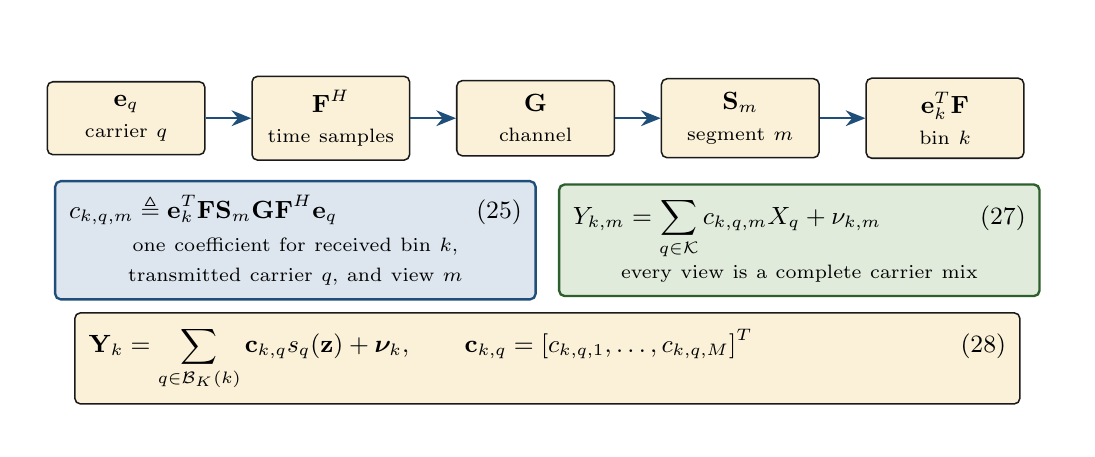
\begin{tikzpicture}[x=1cm,y=1cm]
    \path[use as bounding box] (-6.6,-2.75) rectangle (6.6,2.35);
    \node[card,text width=1.65cm] (eq) at (-5.35,1.20)
      {$\mathbf e_q$\\\scriptsize carrier $q$};
    \node[card,text width=1.65cm] (ifft) at (-2.75,1.20)
      {$\mathbf F^H$\\\scriptsize time samples};
    \node[card,text width=1.65cm] (chan) at (-0.15,1.20)
      {$\mathbf G$\\\scriptsize channel};
    \node[card,text width=1.65cm] (win) at (2.45,1.20)
      {$\mathbf S_m$\\\scriptsize segment $m$};
    \node[card,text width=1.65cm] (fft) at (5.05,1.20)
      {$\mathbf e_k^T\mathbf F$\\\scriptsize bin $k$};
    \draw[bluearr] (eq) -- (ifft);
    \draw[bluearr] (ifft) -- (chan);
    \draw[bluearr] (chan) -- (win);
    \draw[bluearr] (win) -- (fft);

    \node[bluecard,text width=5.75cm] at (-3.20,-0.35) {
      $\displaystyle c_{k,q,m}\triangleq
       \mathbf e_k^T\mathbf F\mathbf S_m\mathbf G\mathbf F^H\mathbf e_q$
      \hfill\textnormal{(25)}\\[0.10em]
      \scriptsize one coefficient for received bin $k$, transmitted carrier $q$, and view $m$};
    \node[goodcard,text width=5.75cm] at (3.20,-0.35) {
      $\displaystyle Y_{k,m}=\sum_{q\in\Kset}c_{k,q,m}X_q+\nu_{k,m}$
      \hfill\textnormal{(27)}\\[0.10em]
      \scriptsize every view is a complete carrier mix};
    \node[card,text width=11.65cm] at (0,-1.85) {
      $\displaystyle \mathbf Y_k=\sum_{q\in\Bset_K(k)}
       \mathbf c_{k,q}s_q(\mathbf z)+\bm\nu_k,
       \qquad
       \mathbf c_{k,q}=[c_{k,q,1},\ldots,c_{k,q,M}]^T$
      \hfill\textnormal{(28)}};
  \end{tikzpicture}
  \bottomnote{The receiver estimates the ICI coefficients; it does not evaluate the time-domain operator $\mathbf G$.  The band retains nearby carrier pairs, while the complete toy calculation keeps all eight carriers.}
\end{frame}

% =====================================================================
% 9. Coefficient sum
% =====================================================================
\begin{frame}{Coefficient sum}
  \centering
  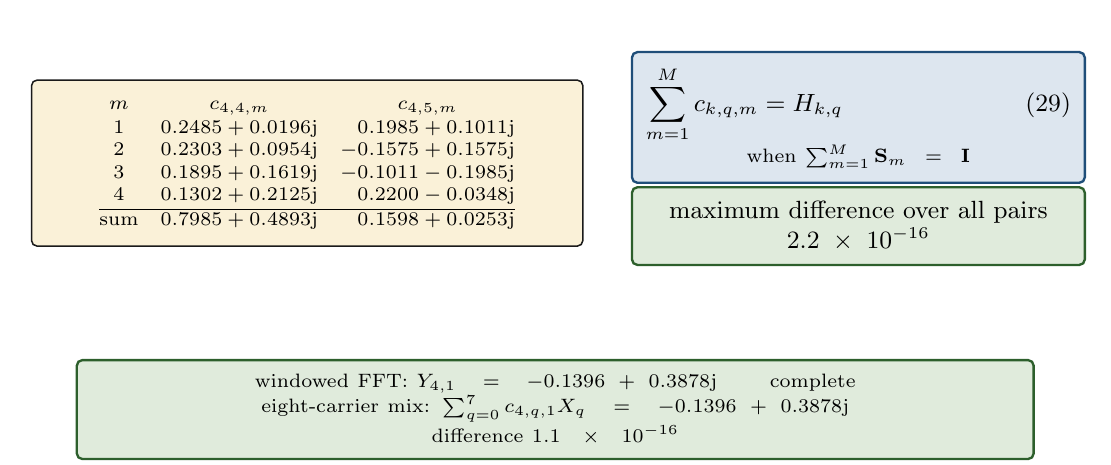
\begin{tikzpicture}[x=1cm,y=1cm]
    \path[use as bounding box] (-6.7,-2.78) rectangle (6.7,2.42);
    \node[card,text width=6.65cm] at (-3.15,0.70) {\scriptsize
      \begin{tabular}{@{}c@{\quad}c@{\quad}c@{}}
      $m$ & $c_{4,4,m}$ & $c_{4,5,m}$\\[0.10em]
      1 & $0.2485+0.0196\mathrm j$ & $\phantom{-}0.1985+0.1011\mathrm j$\\
      2 & $0.2303+0.0954\mathrm j$ & $-0.1575+0.1575\mathrm j$\\
      3 & $0.1895+0.1619\mathrm j$ & $-0.1011-0.1985\mathrm j$\\
      4 & $0.1302+0.2125\mathrm j$ & $\phantom{-}0.2200-0.0348\mathrm j$\\[0.10em]
      \hline
      sum & $0.7985+0.4893\mathrm j$ & $\phantom{-}0.1598+0.0253\mathrm j$
      \end{tabular}};
    \node[bluecard,text width=5.40cm] at (3.85,1.28) {
      $\displaystyle \sum_{m=1}^{M}c_{k,q,m}=H_{k,q}$
      \hfill\textnormal{(29)}\\[-0.02em]
      \scriptsize when $\sum_{m=1}^{M}\mathbf S_m=\mathbf I$};
    \node[goodcard,text width=5.40cm] at (3.85,-0.10)
      {maximum difference over all pairs\\$2.2\times10^{-16}$};
    \node[goodcard,text width=11.80cm] at (0,-2.43) {\scriptsize
      windowed FFT: $Y_{4,1}=-0.1396+0.3878\mathrm j$
      \qquad complete eight-carrier mix:
      $\sum_{q=0}^{7}c_{4,q,1}X_q=-0.1396+0.3878\mathrm j$\\[-0.02em]
      difference $1.1\times10^{-16}$};
  \end{tikzpicture}
  \bottomnote{The per-view coefficients and the channel coefficient are the same channel at two resolutions.  The visible $q=4$ and $q=5$ columns do not assert that the other carrier pairs are zero.}
\end{frame}

% =====================================================================
% 10. Read-out
% =====================================================================
\begin{frame}{The read-out}
  \centering
  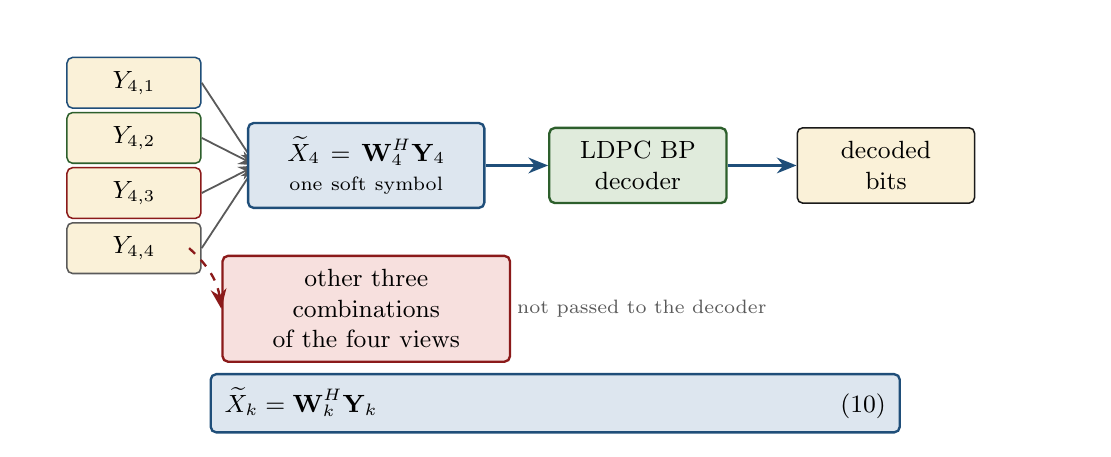
\begin{tikzpicture}[x=1cm,y=1cm]
    \path[use as bounding box] (-6.7,-2.75) rectangle (6.7,2.35);
    \foreach \m/\yy/\col in {1/1.65/accentblue,2/0.95/accentgreen,
                               3/0.25/accentred,4/-0.45/inkgray}{
      \node[card,draw=\col,text width=1.35cm] (y\m) at (-5.35,\yy)
        {$Y_{4,\m}$};
      \draw[grayarr] (y\m.east) -- (-3.80,0.60);
    }
    \node[bluecard,text width=2.65cm] (combine) at (-2.40,0.60)
      {$\widetilde X_4=\mathbf W_4^H\mathbf Y_4$\\[-0.05em]
       \scriptsize one soft symbol};
    \node[goodcard,text width=1.90cm] (bp) at (1.05,0.60)
      {LDPC BP\\decoder};
    \node[card,text width=1.90cm] (bits) at (4.20,0.60)
      {decoded\\bits};
    \draw[bluearr] (combine) -- (bp);
    \draw[bluearr] (bp) -- (bits);
    \node[badcard,text width=3.30cm] (other) at (-2.40,-1.22)
      {other three combinations\\of the four views};
    \draw[redarr,dashed] (-4.65,-0.45) to[bend left=20] (other.west);
    \node[font=\scriptsize,color=inkgray] at (1.10,-1.22)
      {not passed to the decoder};
    \node[bluecard,text width=8.40cm] at (0,-2.42) {
      $\displaystyle \widetilde X_k=\mathbf W_k^H\mathbf Y_k$
      \hfill\textnormal{(10)}};
  \end{tikzpicture}
  \bottomnote{The read-out keeps one combination of a carrier's views for the decoder.  The ICI coefficients are $\mathbf C$; the post-reception combiner is $\mathbf W$.}
\end{frame}

% =====================================================================
% 11. Scalar versus vector
% =====================================================================
\begin{frame}{Scalar and vector}
  \centering
  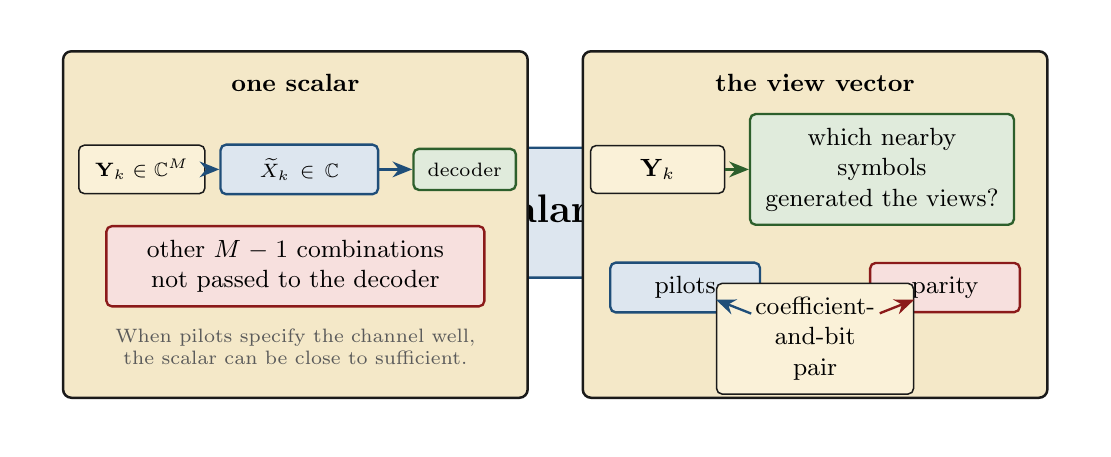
\begin{tikzpicture}[x=1cm,y=1cm]
    \path[use as bounding box] (-6.7,-2.75) rectangle (6.7,2.35);
    \only<1>{%
      \node[bluecard,text width=7.40cm,minimum height=1.65cm,
            font=\Large\bfseries] at (0,0) {Is one scalar enough?};
    }
    \uncover<2->{%
      \draw[panel] (-6.25,-2.35) rectangle (-0.35,2.05);
      \node[font=\small\bfseries] at (-3.30,1.65) {one scalar};
      \node[card,text width=1.25cm,font=\scriptsize] (ys) at (-5.25,0.55)
        {$\mathbf Y_k\in\Cfield^M$};
      \node[bluecard,text width=1.65cm,font=\scriptsize] (ws) at (-3.25,0.55)
        {$\widetilde X_k\in\Cfield$};
      \node[goodcard,text width=0.95cm,font=\scriptsize] (ds) at (-1.15,0.55)
        {decoder};
      \draw[bluearr] (ys) -- (ws);
      \draw[bluearr] (ws) -- (ds);
      \node[badcard,text width=4.45cm] at (-3.30,-0.68)
        {other $M-1$ combinations\\not passed to the decoder};
      \node[font=\scriptsize,color=inkgray,text width=4.9cm,align=center]
        at (-3.30,-1.70)
        {When pilots specify the channel well, the scalar can be close to sufficient.};
    }

    \uncover<3->{%
      \draw[panel] (0.35,-2.35) rectangle (6.25,2.05);
      \node[font=\small\bfseries] at (3.30,1.65) {the view vector};
      \node[card,text width=1.35cm] (yv) at (1.30,0.55) {$\mathbf Y_k$};
      \node[goodcard,text width=3.00cm] (ask) at (4.15,0.55)
        {which nearby symbols\\generated the views?};
      \draw[greenarr] (yv) -- (ask);
      \node[bluecard,text width=1.55cm] (p) at (1.65,-0.95) {pilots};
      \node[badcard,text width=1.55cm] (r) at (4.95,-0.95) {parity};
      \node[card,text width=2.15cm] (cz) at (3.30,-1.60)
        {coefficient-and-bit\\pair};
      \draw[bluearr] (p) -- (cz);
      \draw[redarr] (r) -- (cz);
    }
  \end{tikzpicture}
  \vspace{-0.10cm}
  \uncover<2->{\bottomnote{\scriptsize The scalar is sufficient exactly when $p(\mathbf b\mid\mathbf Y)=p(\mathbf b\mid\widetilde{\mathbf X})$.  The joint search instead keeps the view vectors; pilots constrain the coefficients and parity checks restrict the coded bits.}}
\end{frame}

% 12. Relaxed QPSK
% =====================================================================
\begin{frame}{Relaxed QPSK}
  \centering
  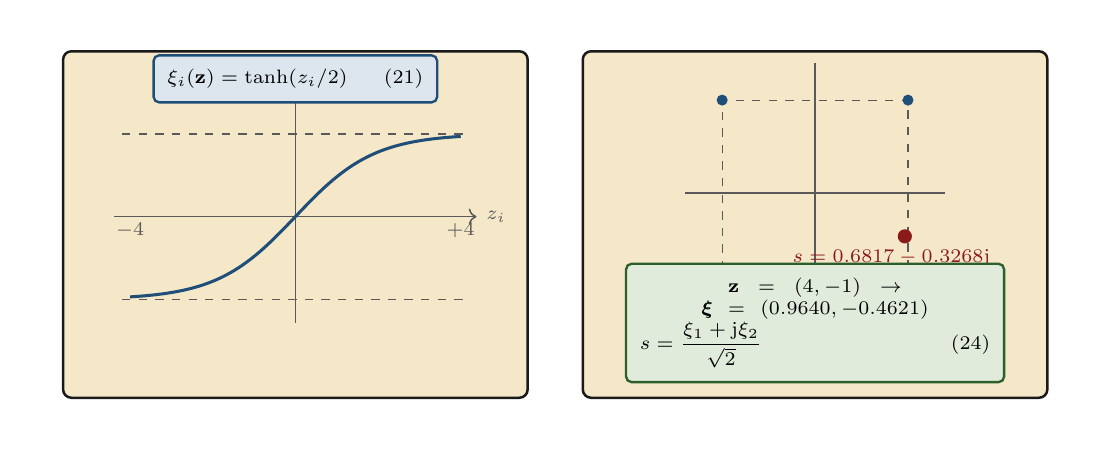
\begin{tikzpicture}[x=1cm,y=1cm]
    \path[use as bounding box] (-6.7,-2.75) rectangle (6.7,2.35);
    \draw[panel] (-6.25,-2.35) rectangle (-0.35,2.05);
    \begin{scope}[shift={(-3.30,-0.05)}]
      \draw[->,line width=0.55pt,color=inkgray] (-2.30,0) -- (2.30,0)
        node[right,font=\scriptsize] {$z_i$};
      \draw[->,line width=0.55pt,color=inkgray] (0,-1.35) -- (0,1.55)
        node[above,font=\scriptsize] {$\xi_i$};
      \draw[dashed,color=inkgray] (-2.20,1.05) -- (2.20,1.05);
      \draw[dashed,color=inkgray] (-2.20,-1.05) -- (2.20,-1.05);
      \draw[line width=1.1pt,color=accentblue,smooth,samples=81,
            domain=-4.20:4.20]
        plot ({0.50*\x},{1.05*tanh(\x/2)});
      \node[bluecard,text width=3.25cm,font=\scriptsize] at (0,1.75)
        {$\xi_i(\mathbf z)=\tanh(z_i/2)$\hfill\textnormal{(21)}};
      \node[font=\scriptsize,color=inkgray] at (-2.10,-0.18) {$-4$};
      \node[font=\scriptsize,color=inkgray] at (2.10,-0.18) {$+4$};
    \end{scope}

    \draw[panel] (0.35,-2.35) rectangle (6.25,2.05);
    \begin{scope}[shift={(3.30,0.25)}]
      \draw[line width=0.5pt,color=inkgray] (-1.65,0) -- (1.65,0);
      \draw[line width=0.5pt,color=inkgray] (0,-1.65) -- (0,1.65);
      \draw[dashed,color=inkgray] (-1.18,-1.18) rectangle (1.18,1.18);
      \foreach \sx/\sy in {1/1,1/-1,-1/1,-1/-1}{
        \fill[accentblue] (1.18*\sx,1.18*\sy) circle (0.07);
      }
      \fill[accentred] (1.14,-0.55) circle (0.09);
      \node[font=\scriptsize,color=accentred,anchor=east] at (2.35,-0.82)
        {$s=0.6817-0.3268\mathrm j$};
      \node[goodcard,text width=4.45cm,font=\scriptsize] at (0,-1.65)
        {$\mathbf z=(4,-1)\rightarrow
          \boldsymbol\xi=(0.9640,-0.4621)$\\
         $\displaystyle s=\frac{\xi_1+\mathrm j\xi_2}{\sqrt2}$
         \hfill\textnormal{(24)}};
    \end{scope}
  \end{tikzpicture}
  \bottomnote{Hard bits give the four quadrature phase-shift keying points.  Relaxed bits move the symbol inside the square and provide a differentiable path.  Pilot carriers keep their known symbols.}
\end{frame}

% =====================================================================
% 13. Pilots
% =====================================================================
\begin{frame}{Pilot constraints}
  \centering
  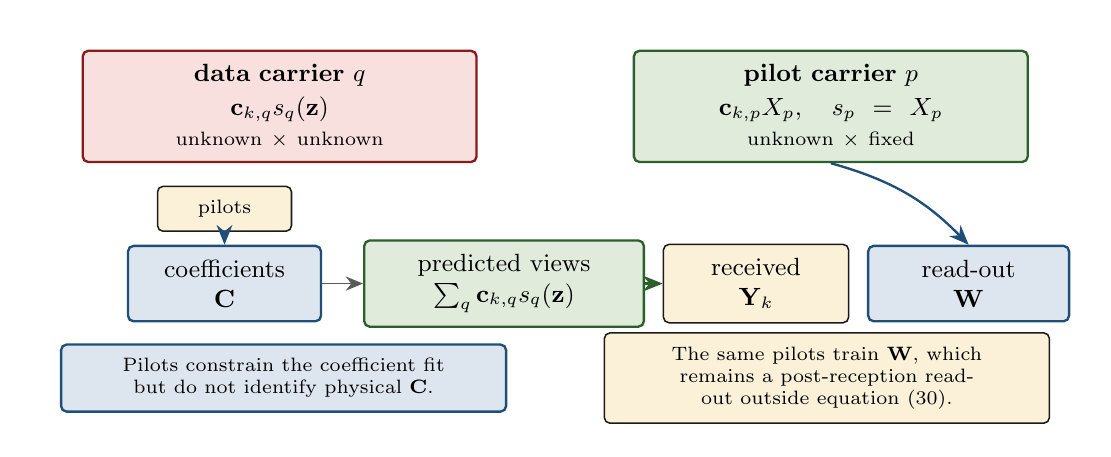
\begin{tikzpicture}[x=1cm,y=1cm]
    \path[use as bounding box] (-6.7,-2.75) rectangle (6.7,2.35);
    \node[badcard,text width=4.65cm] (data) at (-3.50,1.35)
      {\textbf{data carrier $q$}\\[0.12em]
       $\mathbf c_{k,q}s_q(\mathbf z)$\\
       \scriptsize unknown $\times$ unknown};
    \node[goodcard,text width=4.65cm] (pilot) at (3.50,1.35)
      {\textbf{pilot carrier $p$}\\[0.12em]
       $\mathbf c_{k,p}X_p,\quad s_p=X_p$\\
       \scriptsize unknown $\times$ fixed};

    \node[card,text width=1.35cm,font=\scriptsize] (pnode) at (-4.20,0.05)
      {pilots};
    \node[bluecard,text width=2.10cm] (coef) at (-4.20,-0.90)
      {coefficients\\$\mathbf C$};
    \node[goodcard,text width=3.20cm] (model) at (-0.65,-0.90)
      {predicted views\\$\sum_q\mathbf c_{k,q}s_q(\mathbf z)$};
    \node[card,text width=2.00cm] (views) at (2.55,-0.90)
      {received\\$\mathbf Y_k$};
    \node[bluecard,text width=2.20cm] (comb) at (5.25,-0.90)
      {read-out\\$\mathbf W$};
    \draw[bluearr] (pnode) -- (coef);
    \draw[grayarr] (coef) -- (model);
    \draw[greenarr] (model) -- (views);
    \draw[bluearr] (pilot.south) to[bend left=15] (comb.north);

    \node[bluecard,text width=5.30cm,font=\scriptsize] at (-3.45,-2.10)
      {Pilots constrain the coefficient fit but do not identify physical $\mathbf C$.};
    \node[card,text width=5.30cm,font=\scriptsize] at (3.45,-2.10)
      {The same pilots train $\mathbf W$, which remains a post-reception read-out outside equation (30).};
  \end{tikzpicture}
\end{frame}

% =====================================================================
% 14. Parity
% =====================================================================
\begin{frame}{Parity penalty}
  \centering
  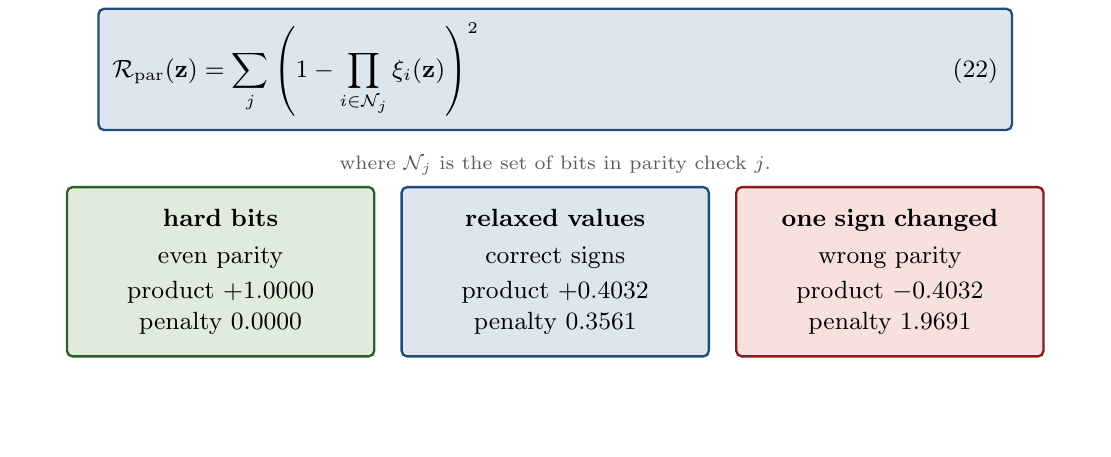
\begin{tikzpicture}[x=1cm,y=1cm]
    \path[use as bounding box] (-6.7,-2.75) rectangle (6.7,2.35);
    \node[bluecard,text width=11.25cm] at (0,1.82) {
      $\displaystyle
       \mathcal R_{\mathrm{par}}(\mathbf z)=
       \sum_j\left(1-\prod_{i\in\mathcal N_j}\xi_i(\mathbf z)\right)^2$
      \hfill\textnormal{(22)}};
    \node[font=\scriptsize,color=inkgray] at (0,0.60)
      {where $\mathcal N_j$ is the set of bits in parity check $j$.};
    \node[goodcard,text width=3.55cm,minimum height=2.15cm] at (-4.25,-0.75)
      {\textbf{hard bits}\\[0.22em]
       even parity\\[0.20em]
       product $+1.0000$\\
       penalty $0.0000$};
    \node[bluecard,text width=3.55cm,minimum height=2.15cm] at (0,-0.75)
      {\textbf{relaxed values}\\[0.22em]
       correct signs\\[0.20em]
       product $+0.4032$\\
       penalty $0.3561$};
    \node[badcard,text width=3.55cm,minimum height=2.15cm] at (4.25,-0.75)
      {\textbf{one sign changed}\\[0.22em]
       wrong parity\\[0.20em]
       product $-0.4032$\\
       penalty $1.9691$};
  \end{tikzpicture}
  \bottomnote{The penalty vanishes on codewords.  Relaxed values with the correct signs remain costly until their magnitudes approach one.}
\end{frame}

% =====================================================================
% 15. Joint objective
% =====================================================================
\begin{frame}{Joint objective}
  \centering
  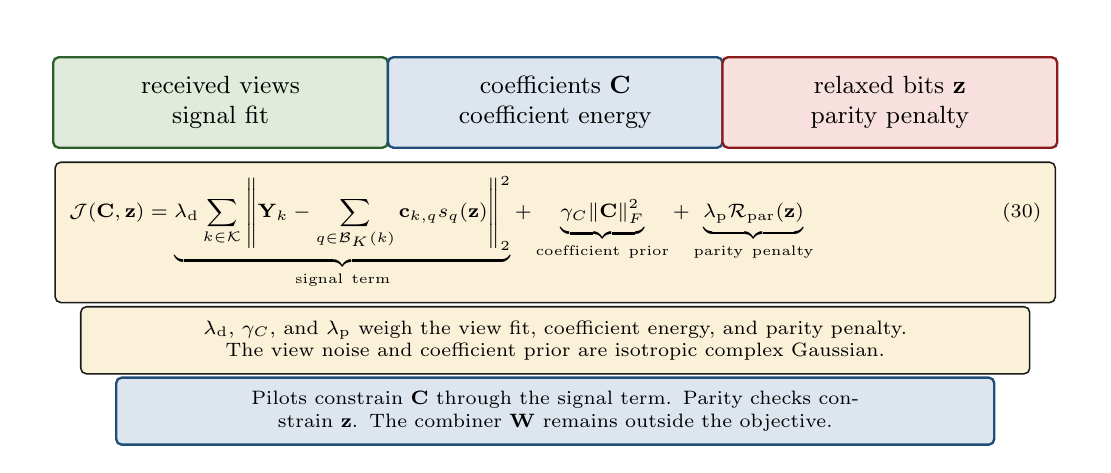
\begin{tikzpicture}[x=1cm,y=1cm]
    \path[use as bounding box] (-6.7,-2.85) rectangle (6.7,2.45);
    \node[goodcard,text width=3.90cm,minimum height=1.15cm] at (-4.25,1.50)
      {received views\\signal fit};
    \uncover<2->{%
      \node[bluecard,text width=3.90cm,minimum height=1.15cm] at (0,1.50)
        {coefficients $\mathbf C$\\coefficient energy};
    }
    \uncover<3->{%
      \node[badcard,text width=3.90cm,minimum height=1.15cm] at (4.25,1.50)
        {relaxed bits $\mathbf z$\\parity penalty};
    }
    \uncover<4->{%
      \node[card,text width=12.35cm,inner sep=5pt] at (0,-0.15) {\scriptsize
        $\displaystyle
         \mathcal J(\mathbf C,\mathbf z)
         =\underbrace{\lambda_{\mathrm d}\sum_{k\in\Kset}
         \left\|\mathbf Y_k-\sum_{q\in\Bset_K(k)}
         \mathbf c_{k,q}s_q(\mathbf z)\right\|_2^2}_{\text{signal term}}
         +\underbrace{\gamma_C\|\mathbf C\|_F^2}_{\text{coefficient prior}}
         +\underbrace{\lambda_{\mathrm p}
         \mathcal R_{\mathrm{par}}(\mathbf z)}_{\text{parity penalty}}$
        \hfill\textnormal{(30)}};
      \node[card,text width=11.70cm,font=\scriptsize] at (0,-1.52)
        {$\lambda_{\mathrm d}$, $\gamma_C$, and $\lambda_{\mathrm p}$ weigh the view fit, coefficient energy, and parity penalty.  The view noise and coefficient prior are isotropic complex Gaussian.};
      \node[bluecard,text width=10.80cm,font=\scriptsize] at (0,-2.42)
        {Pilots constrain $\mathbf C$ through the signal term.  Parity checks constrain $\mathbf z$.  The combiner $\mathbf W$ remains outside the objective.};
    }
  \end{tikzpicture}
\end{frame}

% =====================================================================
% 16. Separate numerical checks
% =====================================================================
\begin{frame}{Separate checks}
  \centering
  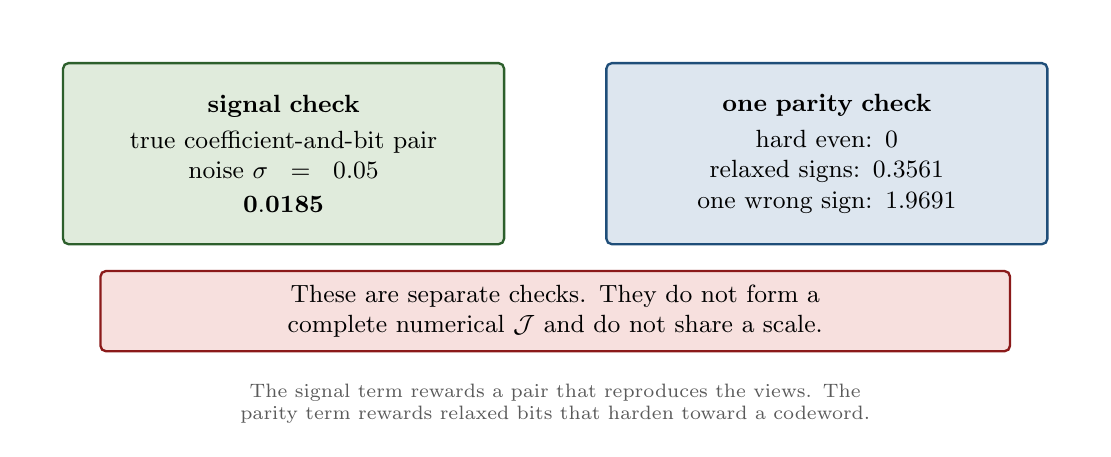
\begin{tikzpicture}[x=1cm,y=1cm]
    \path[use as bounding box] (-6.7,-2.75) rectangle (6.7,2.35);
    \node[goodcard,text width=5.25cm,minimum height=2.30cm] at (-3.45,0.75)
      {\textbf{signal check}\\[0.22em]
       true coefficient-and-bit pair\\
       noise $\sigma=0.05$\\[0.12em]
       $\mathbf{0.0185}$};
    \node[bluecard,text width=5.25cm,minimum height=2.30cm] at (3.45,0.75)
      {\textbf{one parity check}\\[0.22em]
       hard even: $0$\\
       relaxed signs: $0.3561$\\
       one wrong sign: $1.9691$};
    \node[badcard,text width=11.20cm] at (0,-1.25)
      {These are separate checks.  They do not form a complete numerical $\mathcal J$ and do not share a scale.};
    \node[font=\scriptsize,color=inkgray,text width=11.0cm,align=center]
      at (0,-2.42)
      {The signal term rewards a pair that reproduces the views.  The parity term rewards relaxed bits that harden toward a codeword.};
  \end{tikzpicture}
\end{frame}

% =====================================================================
% 17. Local gradient example
% =====================================================================
\begin{frame}{Local gradient check}
  \centering
  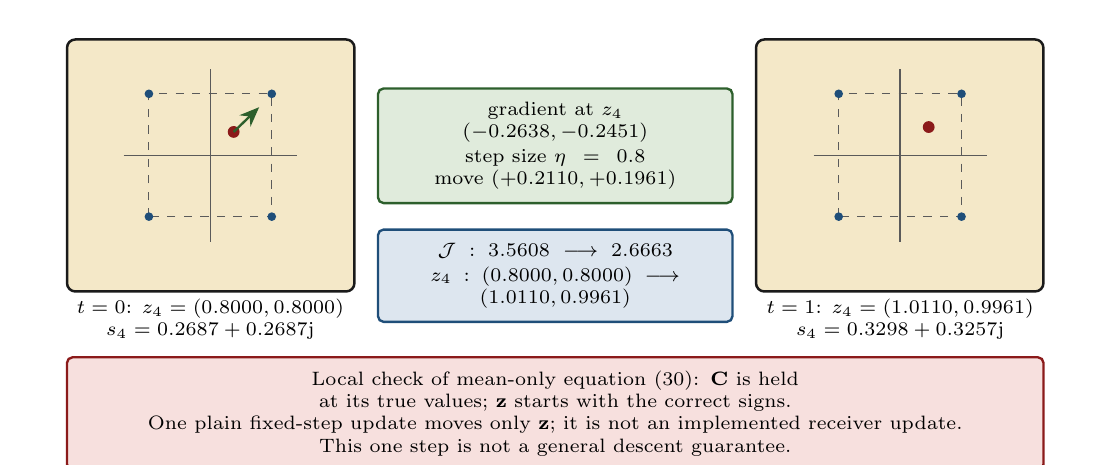
\begin{tikzpicture}[x=1cm,y=1cm]
    \path[use as bounding box] (-6.7,-2.80) rectangle (6.7,2.40);
    \draw[panel] (-6.20,-0.95) rectangle (-2.55,2.25);
    \begin{scope}[shift={(-4.38,0.78)}]
      \draw[line width=0.45pt,color=inkgray] (-1.10,0) -- (1.10,0);
      \draw[line width=0.45pt,color=inkgray] (0,-1.10) -- (0,1.10);
      \draw[dashed,color=inkgray] (-0.78,-0.78) rectangle (0.78,0.78);
      \foreach \sx/\sy in {1/1,1/-1,-1/1,-1/-1}{
        \fill[accentblue] (0.78*\sx,0.78*\sy) circle (0.055);
      }
      \fill[accentred] (0.296,0.296) circle (0.075);
      \uncover<2->{\draw[greenarr] (0.296,0.296) -- (0.62,0.61);}
    \end{scope}
    \node[font=\scriptsize,align=center] at (-4.38,-1.30)
      {$t=0$: $z_4=(0.8000,0.8000)$\\
       $s_4=0.2687+0.2687\mathrm j$};

    \uncover<2->{%
      \node[goodcard,text width=4.15cm,font=\scriptsize] at (0,0.90)
        {gradient at $z_4$\\$(-0.2638,-0.2451)$\\[0.10em]
         step size $\eta=0.8$\\move $(+0.2110,+0.1961)$};
    }
    \uncover<3->{%
      \node[bluecard,text width=4.15cm,font=\scriptsize] at (0,-0.75)
        {$\mathcal J: 3.5608\longrightarrow2.6663$\\[0.10em]
         $z_4: (0.8000,0.8000)\longrightarrow(1.0110,0.9961)$};
    }

    \uncover<3->{%
      \draw[panel] (2.55,-0.95) rectangle (6.20,2.25);
      \begin{scope}[shift={(4.38,0.78)}]
        \draw[line width=0.45pt,color=inkgray] (-1.10,0) -- (1.10,0);
        \draw[line width=0.45pt,color=inkgray] (0,-1.10) -- (0,1.10);
        \draw[dashed,color=inkgray] (-0.78,-0.78) rectangle (0.78,0.78);
        \foreach \sx/\sy in {1/1,1/-1,-1/1,-1/-1}{
          \fill[accentblue] (0.78*\sx,0.78*\sy) circle (0.055);
        }
        \fill[accentred] (0.363,0.358) circle (0.075);
      \end{scope}
      \node[font=\scriptsize,align=center] at (4.38,-1.30)
        {$t=1$: $z_4=(1.0110,0.9961)$\\
         $s_4=0.3298+0.3257\mathrm j$};
    }

    \node[badcard,text width=12.05cm,font=\scriptsize] at (0,-2.50)
      {Local check of mean-only equation (30): $\mathbf C$ is held at its true values; $\mathbf z$ starts with the correct signs.\\
       One plain fixed-step update moves only $\mathbf z$; it is not an implemented receiver update.\\
       This one step is not a general descent guarantee.};
  \end{tikzpicture}
\end{frame}

% =====================================================================
% 18. Five-receiver overview
% =====================================================================
\begin{frame}{Five receivers}
  \centering
  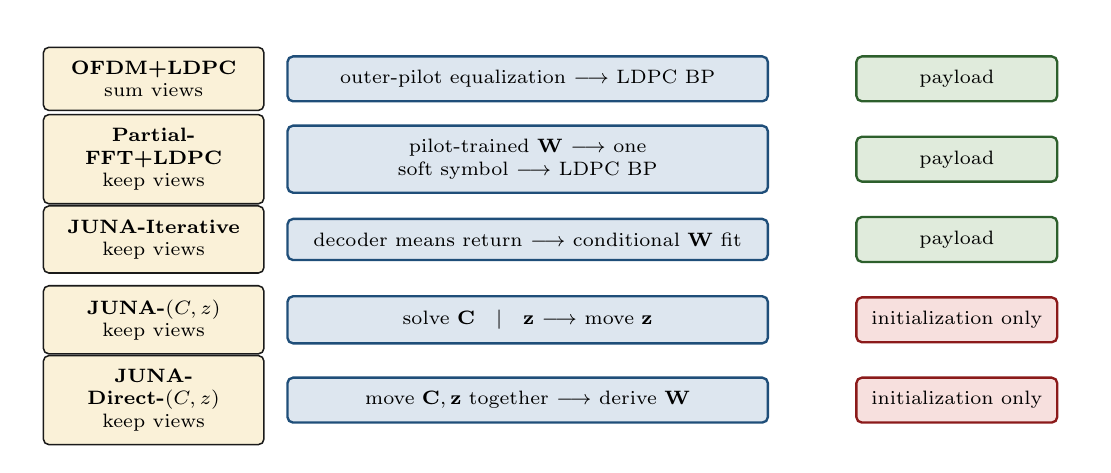
\begin{tikzpicture}[x=1cm,y=1cm]
    \path[use as bounding box] (-6.7,-2.85) rectangle (6.7,2.45);
    \node[card,text width=2.45cm,font=\scriptsize] at (-5.10,1.80)
      {\textbf{OFDM+LDPC}\\sum views};
    \node[bluecard,text width=5.75cm,font=\scriptsize] at (-0.35,1.80)
      {outer-pilot equalization $\longrightarrow$ LDPC BP};
    \node[goodcard,text width=2.20cm,font=\scriptsize] at (5.10,1.80)
      {payload};

    \node[card,text width=2.45cm,font=\scriptsize] at (-5.10,0.78)
      {\textbf{Partial-FFT+LDPC}\\keep views};
    \node[bluecard,text width=5.75cm,font=\scriptsize] at (-0.35,0.78)
      {pilot-trained $\mathbf W$ $\longrightarrow$ one soft symbol $\longrightarrow$ LDPC BP};
    \node[goodcard,text width=2.20cm,font=\scriptsize] at (5.10,0.78)
      {payload};

    \node[card,text width=2.45cm,font=\scriptsize] at (-5.10,-0.24)
      {\textbf{JUNA-Iterative}\\keep views};
    \node[bluecard,text width=5.75cm,font=\scriptsize] at (-0.35,-0.24)
      {decoder means return $\longrightarrow$ conditional $\mathbf W$ fit};
    \node[goodcard,text width=2.20cm,font=\scriptsize] at (5.10,-0.24)
      {payload};

    \node[card,text width=2.45cm,font=\scriptsize] at (-5.10,-1.26)
      {\textbf{JUNA-$(C,z)$}\\keep views};
    \node[bluecard,text width=5.75cm,font=\scriptsize] at (-0.35,-1.26)
      {solve $\mathbf C\mid\mathbf z$ $\longrightarrow$ move $\mathbf z$};
    \node[badcard,text width=2.20cm,font=\scriptsize] at (5.10,-1.26)
      {initialization only};

    \node[card,text width=2.45cm,font=\scriptsize] at (-5.10,-2.28)
      {\textbf{JUNA-Direct-$(C,z)$}\\keep views};
    \node[bluecard,text width=5.75cm,font=\scriptsize] at (-0.35,-2.28)
      {move $\mathbf C,\mathbf z$ together $\longrightarrow$ derive $\mathbf W$};
    \node[badcard,text width=2.20cm,font=\scriptsize] at (5.10,-2.28)
      {initialization only};
  \end{tikzpicture}
  \bottomnote{The first two receivers separate demodulation from decoding.  The next three use decoder information or relaxed coded bits during symbol estimation.}
\end{frame}

% =====================================================================
% 19. JUNA-Iterative
% =====================================================================
\begin{frame}{JUNA-Iterative}
  \centering
  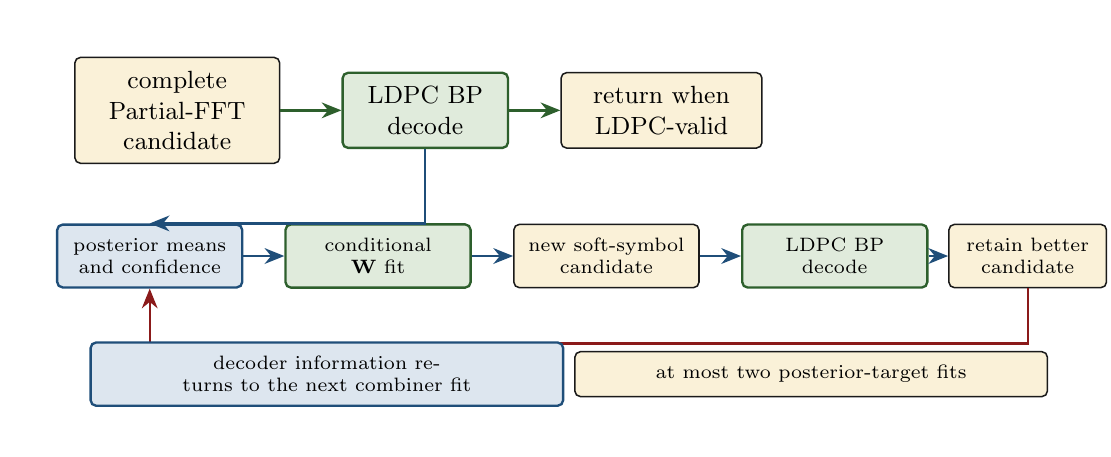
\begin{tikzpicture}[x=1cm,y=1cm]
    \path[use as bounding box] (-6.7,-2.75) rectangle (6.7,2.35);
    \node[card,text width=2.25cm] (start) at (-4.80,1.30)
      {complete Partial-FFT\\candidate};
    \node[goodcard,text width=1.75cm] (decode0) at (-1.65,1.30)
      {LDPC BP\\decode};
    \node[card,text width=2.20cm] (return) at (1.35,1.30)
      {return when\\LDPC-valid};
    \draw[greenarr] (start) -- (decode0);
    \draw[greenarr] (decode0) -- (return);

    \node[bluecard,text width=2.00cm,font=\scriptsize] (mean) at (-5.15,-0.55)
      {posterior means\\and confidence};
    \node[goodcard,text width=2.00cm,font=\scriptsize] (fit) at (-2.25,-0.55)
      {conditional\\$\mathbf W$ fit};
    \node[card,text width=2.00cm,font=\scriptsize] (soft) at (0.65,-0.55)
      {new soft-symbol\\candidate};
    \node[goodcard,text width=2.00cm,font=\scriptsize] (decode) at (3.55,-0.55)
      {LDPC BP\\decode};
    \node[card,text width=1.65cm,font=\scriptsize] (best) at (6.00,-0.55)
      {retain better\\candidate};
    \draw[bluearr] (decode0.south) |- (mean.north);
    \draw[bluearr] (mean) -- (fit);
    \draw[bluearr] (fit) -- (soft);
    \draw[bluearr] (soft) -- (decode);
    \draw[bluearr] (decode) -- (best);
    \draw[redarr] (best.south) -- ++(0,-0.70) -| (mean.south);

    \node[bluecard,text width=5.65cm,font=\scriptsize] at (-2.90,-2.05)
      {decoder information returns to the next combiner fit};
    \node[card,text width=5.65cm,font=\scriptsize] at (3.25,-2.05)
      {at most two posterior-target fits};
  \end{tikzpicture}
  \vspace{-0.10cm}
  \bottomnote{\scriptsize Like turbo equalization, JUNA-Iterative repeats equalization and decoding.  This exchange approximates the joint loop, but forms no $\mathbf C$, has no free $\mathbf z$, and never evaluates equation (30).}
\end{frame}

% =====================================================================
% 20. JUNA-(C,z)
% =====================================================================
\begin{frame}{JUNA-$(C,z)$}
  \centering
  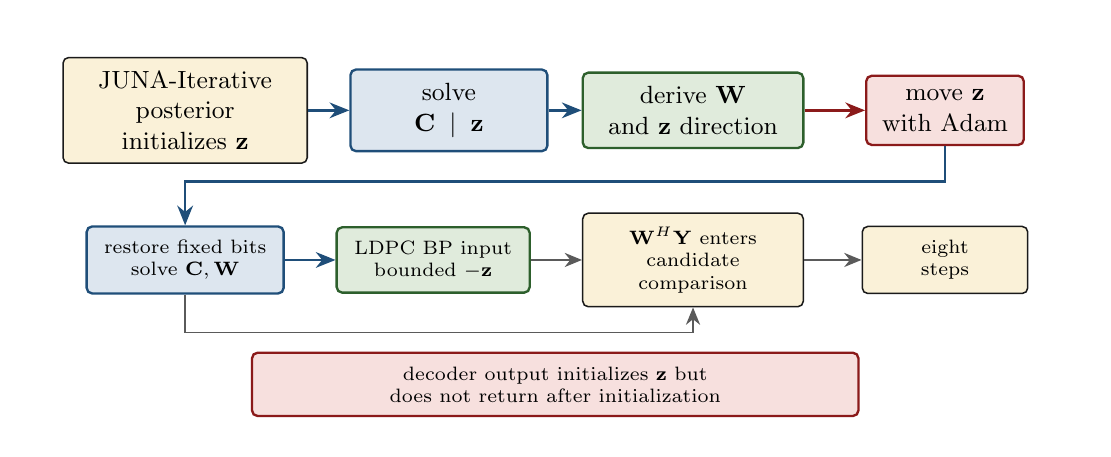
\begin{tikzpicture}[x=1cm,y=1cm]
    \path[use as bounding box] (-6.7,-2.75) rectangle (6.7,2.35);
    \node[card,text width=2.75cm] (initial) at (-4.70,1.30)
      {JUNA-Iterative posterior\\initializes $\mathbf z$};
    \node[bluecard,text width=2.15cm] (c) at (-1.35,1.30)
      {solve\\$\mathbf C\mid\mathbf z$};
    \node[goodcard,text width=2.45cm] (w) at (1.75,1.30)
      {derive $\mathbf W$\\and $\mathbf z$ direction};
    \node[badcard,text width=1.65cm] (adam) at (4.95,1.30)
      {move $\mathbf z$\\with Adam};
    \draw[bluearr] (initial) -- (c);
    \draw[bluearr] (c) -- (w);
    \draw[redarr] (w) -- (adam);

    \node[bluecard,text width=2.15cm,font=\scriptsize] (again) at (-4.70,-0.60)
      {restore fixed bits\\solve $\mathbf C,\mathbf W$};
    \node[goodcard,text width=2.10cm,font=\scriptsize] (bp) at (-1.55,-0.60)
      {LDPC BP input\\bounded $-\mathbf z$};
    \node[card,text width=2.45cm,font=\scriptsize] (score) at (1.75,-0.60)
      {$\mathbf W^H\mathbf Y$ enters\\candidate comparison};
    \node[card,text width=1.75cm,font=\scriptsize] (eight) at (4.95,-0.60)
      {eight\\steps};
    \draw[bluearr] (adam.south) -- ++(0,-0.45) -| (again.north);
    \draw[bluearr] (again) -- (bp);
    \draw[grayarr] (again.south) -- ++(0,-0.48) -| (score.south);
    \draw[grayarr] (bp) -- (score);
    \draw[grayarr] (score) -- (eight);
    \node[badcard,text width=7.35cm,font=\scriptsize] at (0,-2.18)
      {decoder output initializes $\mathbf z$ but does not return after initialization};
  \end{tikzpicture}
  \vspace{-0.10cm}
  \bottomnote{\scriptsize The coefficient and relaxed-bit blocks are motivated by equation (30).  The executed frame cost is given with the experiment settings and is not identical to equation (30).}
\end{frame}

% =====================================================================
% 21. JUNA-Direct-(C,z)
% =====================================================================
\begin{frame}{JUNA-Direct-$(C,z)$}
  \centering
  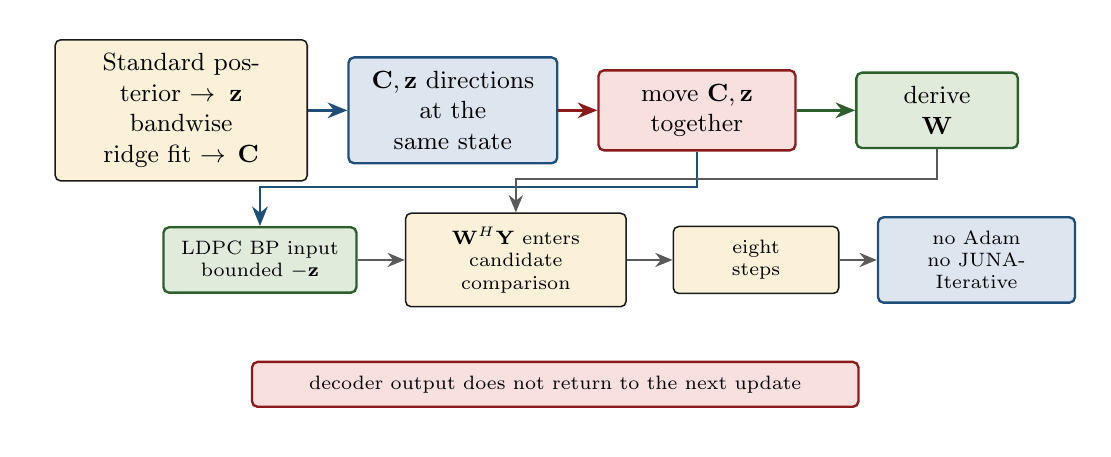
\begin{tikzpicture}[x=1cm,y=1cm]
    \path[use as bounding box] (-6.7,-2.75) rectangle (6.7,2.35);
    \node[card,text width=2.85cm] (initial) at (-4.75,1.30)
      {Standard posterior $\to\mathbf z$\\bandwise ridge fit $\to\mathbf C$};
    \node[bluecard,text width=2.30cm] (dir) at (-1.30,1.30)
      {$\mathbf C,\mathbf z$ directions\\at the same state};
    \node[badcard,text width=2.15cm] (move) at (1.80,1.30)
      {move $\mathbf C,\mathbf z$\\together};
    \node[goodcard,text width=1.70cm] (w) at (4.85,1.30)
      {derive\\$\mathbf W$};
    \draw[bluearr] (initial) -- (dir);
    \draw[redarr] (dir) -- (move);
    \draw[greenarr] (move) -- (w);

    \node[goodcard,text width=2.10cm,font=\scriptsize] (bp) at (-3.75,-0.60)
      {LDPC BP input\\bounded $-\mathbf z$};
    \node[card,text width=2.45cm,font=\scriptsize] (score) at (-0.50,-0.60)
      {$\mathbf W^H\mathbf Y$ enters\\candidate comparison};
    \node[card,text width=1.75cm,font=\scriptsize] (eight) at (2.55,-0.60)
      {eight\\steps};
    \node[bluecard,text width=2.15cm,font=\scriptsize] (none) at (5.35,-0.60)
      {no Adam\\no JUNA-Iterative};
    \draw[bluearr] (move.south) -- ++(0,-0.45) -| (bp.north);
    \draw[grayarr] (w.south) -- ++(0,-0.38) -| (score.north);
    \draw[grayarr] (bp) -- (score);
    \draw[grayarr] (score) -- (eight);
    \draw[grayarr] (eight) -- (none);
    \node[badcard,text width=7.35cm,font=\scriptsize] at (0,-2.18)
      {decoder output does not return to the next update};
  \end{tikzpicture}
  \bottomnote{JUNA-Direct-$(C,z)$ moves the coefficient and relaxed-bit variables together.  The weights are derived from the updated coefficients and remain outside equation (30).}
\end{frame}

% =====================================================================
% 22. Takeaway
% =====================================================================
\begin{frame}{Takeaway}
  \centering
  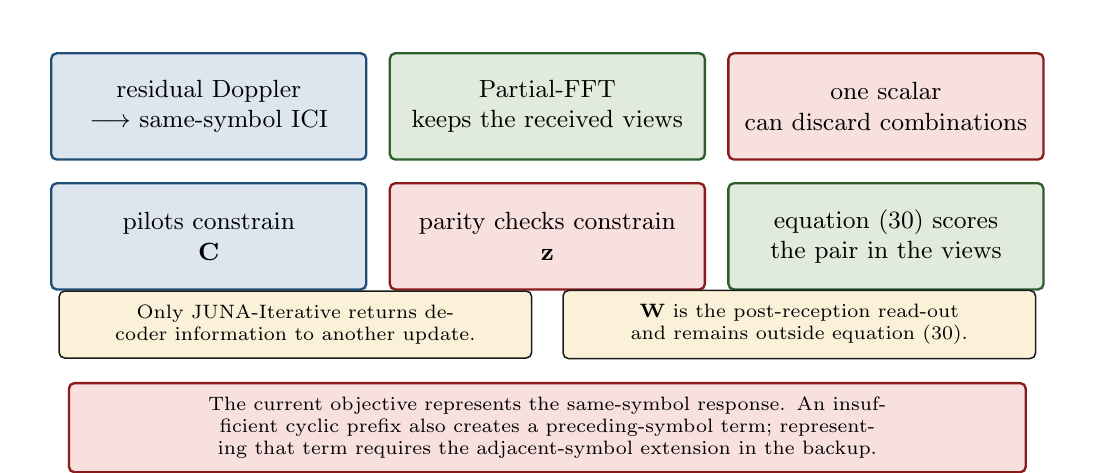
\begin{tikzpicture}[x=1cm,y=1cm]
    \path[use as bounding box] (-6.6,-2.85) rectangle (6.6,2.45);
    \node[bluecard,text width=3.65cm,minimum height=1.35cm] at (-4.30,1.45)
      {residual Doppler\\$\longrightarrow$ same-symbol ICI};
    \node[goodcard,text width=3.65cm,minimum height=1.35cm] at (0,1.45)
      {Partial-FFT\\keeps the received views};
    \node[badcard,text width=3.65cm,minimum height=1.35cm] at (4.30,1.45)
      {one scalar\\can discard combinations};

    \node[bluecard,text width=3.65cm,minimum height=1.35cm] at (-4.30,-0.20)
      {pilots constrain\\$\mathbf C$};
    \node[badcard,text width=3.65cm,minimum height=1.35cm] at (0,-0.20)
      {parity checks constrain\\$\mathbf z$};
    \node[goodcard,text width=3.65cm,minimum height=1.35cm] at (4.30,-0.20)
      {equation (30) scores\\the pair in the views};

    \node[card,text width=5.65cm,font=\scriptsize] at (-3.20,-1.32)
      {Only JUNA-Iterative returns decoder information to another update.};
    \node[card,text width=5.65cm,font=\scriptsize] at (3.20,-1.32)
      {$\mathbf W$ is the post-reception read-out and remains outside equation (30).};
    \node[badcard,text width=11.80cm,font=\scriptsize] at (0,-2.63)
      {The current objective represents the same-symbol response.  An insufficient cyclic prefix also creates a preceding-symbol term; representing that term requires the adjacent-symbol extension in the backup.};
  \end{tikzpicture}
\end{frame}

\pdfstringdefDisableCommands{\def\translate#1{#1}}
\appendix

% =====================================================================
% Backup 1. Adjacent-symbol extension
% =====================================================================
\begin{frame}{Adjacent-symbol extension}
  \centering
  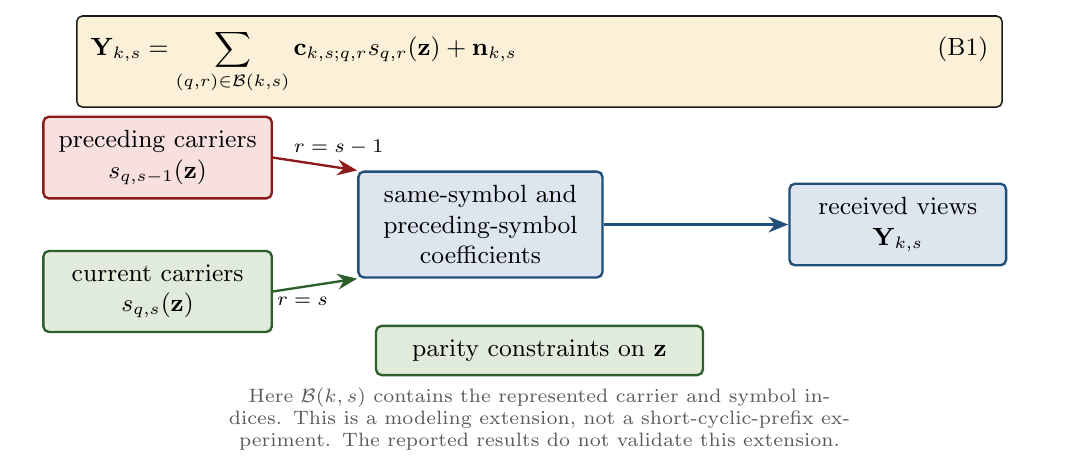
\begin{tikzpicture}[x=1cm,y=1cm]
    \path[use as bounding box] (-6.5,-2.80) rectangle (6.5,2.45);
    \node[badcard,text width=2.55cm] (prev) at (-4.85,0.80)
      {preceding carriers\\$s_{q,s-1}(\mathbf z)$};
    \node[goodcard,text width=2.55cm] (curr) at (-4.85,-0.90)
      {current carriers\\$s_{q,s}(\mathbf z)$};
    \node[bluecard,text width=2.75cm] (resp) at (-0.75,-0.05)
      {same-symbol and\\preceding-symbol\\coefficients};
    \node[bluecard,text width=2.40cm] (out) at (4.55,-0.05)
      {received views\\$\mathbf Y_{k,s}$};
    \draw[redarr] (prev.east) -- node[above,pos=0.78,yshift=1pt,font=\scriptsize] {$r=s-1$} (resp.north west);
    \draw[greenarr] (curr.east) -- node[below,pos=0.35,font=\scriptsize] {$r=s$} (resp.south west);
    \draw[bluearr] (resp) -- (out);
    \node[card,text width=11.40cm] at (0,2.02) {
      $\displaystyle
       \mathbf Y_{k,s}=\sum_{(q,r)\in\Bset(k,s)}
       \mathbf c_{k,s;q,r}s_{q,r}(\mathbf z)+\mathbf n_{k,s}$
      \hfill\textnormal{(B1)}};
    \node[goodcard,text width=3.80cm] at (0,-1.65)
      {parity constraints on $\mathbf z$};
    \node[font=\scriptsize,color=inkgray,text width=11.40cm,align=center]
      at (0,-2.52)
      {Here $\Bset(k,s)$ contains the represented carrier and symbol indices.  This is a modeling extension, not a short-cyclic-prefix experiment.  The reported results do not validate this extension.};
  \end{tikzpicture}
\end{frame}

% =====================================================================
% Backup 2. Posterior variance
% =====================================================================
\begin{frame}{Posterior-variance alternative}
  \centering
  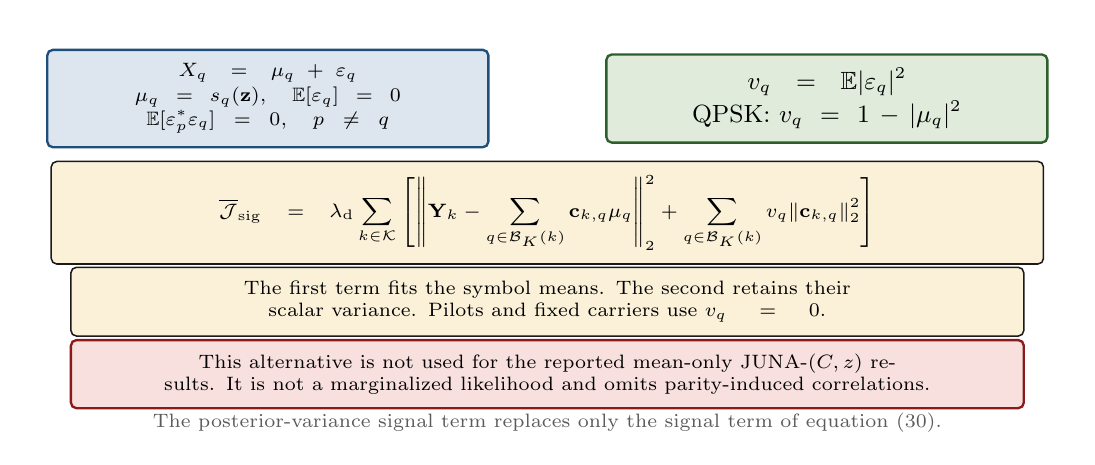
\begin{tikzpicture}[x=1cm,y=1cm]
    \path[use as bounding box] (-6.6,-2.80) rectangle (6.6,2.40);
    \node[bluecard,text width=5.25cm,font=\scriptsize] at (-3.55,1.50)
      {$X_q=\mu_q+\varepsilon_q$\\[0.10em]
       $\mu_q=s_q(\mathbf z),\quad \E[\varepsilon_q]=0$\\[0.08em]
       $\E[\varepsilon_p^*\varepsilon_q]=0,\quad p\ne q$};
    \node[goodcard,text width=5.25cm] at (3.55,1.50)
      {$v_q=\E|\varepsilon_q|^2$\\[0.10em]
       QPSK: $v_q=1-|\mu_q|^2$};
    \node[card,text width=12.25cm,inner sep=5pt] at (0,0.05) {\scriptsize
      $\displaystyle
       \overline{\mathcal J}_{\mathrm{sig}}
       =\lambda_{\mathrm d}\sum_{k\in\Kset}
       \left[
       \left\|\mathbf Y_k-
       \sum_{q\in\Bset_K(k)}\mathbf c_{k,q}\mu_q\right\|_2^2
       +\sum_{q\in\Bset_K(k)}v_q\|\mathbf c_{k,q}\|_2^2
       \right]$
      };
    \node[card,text width=11.75cm,font=\scriptsize] at (0,-1.08)
      {The first term fits the symbol means.  The second retains their scalar variance.  Pilots and fixed carriers use $v_q=0$.};
    \node[badcard,text width=11.75cm,font=\scriptsize] at (0,-2.00)
      {This alternative is not used for the reported mean-only JUNA-$(C,z)$ results.  It is not a marginalized likelihood and omits parity-induced correlations.};
    \node[font=\scriptsize,color=inkgray] at (0,-2.62)
      {The posterior-variance signal term replaces only the signal term of equation (30).};
  \end{tikzpicture}
\end{frame}

\end{document}
